\documentclass[12pt,a4paper]{article} 
\usepackage[T1]{fontenc}
\usepackage[francais]{babel}
\usepackage[latin1]{inputenc}
\usepackage{amsmath}
\usepackage{amssymb} %pour des symboles mathematique
\usepackage{graphicx} 
\usepackage{epstopdf} %pour utiliser les .eps
\usepackage{url}
\usepackage{fancyhdr}
\usepackage{fullpage}
\usepackage{array}
\usepackage[table]{xcolor} %pour les couleurs
\usepackage{multicol}
\usepackage[babel=true]{csquotes} %pour les citations
\usepackage{hyperref}
\usepackage{float} 
\usepackage{adjustbox} %pour resizer les tableaux

%%%% pour l'insertion de code %%%%%
\usepackage{listings}
\usepackage{color}

\definecolor{dkgreen}{rgb}{0,0.6,0}
\definecolor{gray}{rgb}{0,0,0}
\definecolor{mauve}{rgb}{0,0,0}

\lstset{emph={%  
    float, %
    },emphstyle={\color{gray}\bfseries}%
}%

\lstset{frame=tb,
  language=Matlab,
  aboveskip=3mm,
  belowskip=3mm,
  showstringspaces=false,
  columns=flexible,
  basicstyle={\small\ttfamily},
  numbers=none,
  numberstyle=\tiny\color{gray},
  keywordstyle=\color{black},
  commentstyle=\color{dkgreen},
  stringstyle=\color{black},
  identifierstyle=\color{mauve},
  breaklines=true,
  breakatwhitespace=true
  tabsize=3
}

%%%%%%%%%%%%%%%%%%%%%%

%\pagestyle{myheadings}
%\markright{Tableau blanc interactif}

\title{\LARGE \textbf{Project - The Game Cube\textregistered}\\
	\bigskip
	\bigskip
	\large Technologies for human-computer interactions}
\author{Aina Rasolonjatovo Alain Nary Andriambelo \\ Samuel Constantino}
\date{Spring 2014}

\parindent=0cm
\parskip=6pt

\begin{document}
	\maketitle

%%%%%%%%%%%%%%%%%%%%%%%

\section{Introduction}

The goal of this project is to build a game exploring original human-machine interactions. For that, we used a galvanic skin response (GSR) sensor as the main mean of interaction and the \texttt{Blender} 3d software to create the game. In our project, we use the GSR data - which measures skin conductance - as an indicator for stress and arousal. The goal of the game is for the player to manage her stress level and relax. Aina did the sensor and 3d rendering part and Samuel did the game programming and data processing.

\section{Method}

\subsection{Sensor data}

We started from the premise that the GSR sensor could be used as an indicator of excitement. Psychological arousal is linked with nervous activity that changes skin conductance. However, data from the GSR sensor isn't necessarily stable and skin conductance is subject to sudden changes (spikes) that doesn't reflect a general state of being.

In our game, we used a statistical analysis technique called \textbf{moving average} to smooth out the data. The advantage of the moving average is that it reduces the impact of spikes but still preserves long-term tendencies, similarly to a low-pass filter. This technique is usually used in finance and economy to represent trends over time, which is what we want with real-time acquisition of data. More precisely, we use a weighted moving average (WMA) which gives more importance to the oldest data and prevent influence from sudden spikes. It has the following formula : 

\begin{equation}
\text{WMA} = \frac{n * p_n + (n - 1) * p_{n-1} + ... + 1 * p_{1}}{n + (n-1) + ... + 1}
\end{equation}

Where $n$ is the number of data in a queue, $p_x$ is some GSR value at point $x$ in the queue and $p_n$ is the oldest data in the queue. Our moving average is calculated for each new received data by adding it to a queue of size $n=20$.

Here is an illustration of the smoothing done by moving average\footnote{Image taken from : \\ \hyperref[]{http://support2.dundas.com/OnlineDocumentation/WinChart2003/WeightedMovingAverage.html}} :

\begin{figure}[H] 
\centering
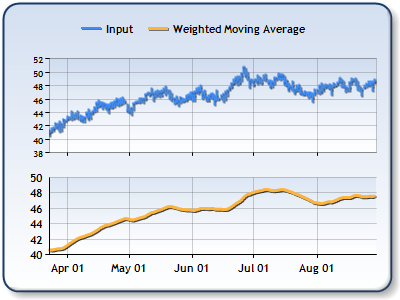
\includegraphics{WeightedMovingAverage.png}
\caption{Exemple of smoothing with weighted moving average.}
\end{figure}

The disadvantage of this technique is that there is a slight delay when trends shift, because the first few points do not have enough weight to influence the average yet.

\subsection{Game design}

The game consists of a cube rotating in the middle of the screen. The cube rotates according to the player's state. Getting excited results in a fast acceleration while being calm makes the cube slow down. By controlling her ``emotions'' (or at least her excitation), the player can then control the speed of the rotation.

%2 modes
The game has two modes of play, \texttt{Relaxation mode} and \texttt{Challenge mode}. 

Relaxation mode only consists of the rotating cube inside an environment without any time restriction. There is no objective in this mode. It can be used as an introduction to the game, to familiarize the player to the controls.

Challenge mode is about winning as much points as possible by controlling the cube's rotation and completing missions before the end of the time allocated. Since the game is about controlling the stress of a player, two elements are used during the game : Mission where the player have to change his stress to have benefices and Event that disrupt the player.
%Challenge mode : introduction

%Challenge mode : Mission
In Challenge mode, missions are based on controlling the cube's rotation speed (with goals like not exceeding a given speed value). Completing a mission grants the player points for her score, and extends the time before the game is over. Failing a mission won't have any effect, besides the time lost during the mission. Up to two missions can appears at the same time. After the time limit is elapsed, the game is over. The missions are randomized  by shuffling a list of possible missions to prevent repetition.

%[IMAGE DU JEU ICI?]

%Challenge mode : Event
While playing Challenge mode some special events may modify the interface or the cube's environment in order to destabilize the player, which can make some missions harder. For example, the cube can suddenly stop moving, although the stress of the player still affects the results of the missions. These events occur randomly with a low probability and may not happen at all during a game.

%way to understand how game works
%how rythme works
%relax and sooth 
%
%challenge mode,
%time limit, playing as long as possible
%win more time by completing missions
%once finished, score (calculated according to missions)
%mission types - 
%slow down, not variate, etc
%randomized mission in a shuffled list (to prevent many repetitions)
%special events to distract player - jump scare 


\subsection{Blender}

%send data over socket
At the start of the game, we instantiate sockets between blender and the GSR device to establish a connection. We use the UDP protocol since the data from the GSR to the game is numerous. Unlike the TCP/IP protocol there is no problem if some data is lost and no synchronization is required. Blender only sends a starting and stopping order to the game (at the start and end respectively) to receive data.


%cube
In Blender, the cube is a mesh cube that has a modifier applied to it. It consists of a sphere "expended" to the border of the cube, to every direction so that the corner and the edges are smoother.

%Image du cube sans modifier > image du cube avec modifier?

%HUD position
%movement camera, 
During challenge mode, a head-up display (HUD) shows information to the player concerning the time left, the on-going missions, current score and the cube's speed. The HUD is locked to the camera so that it follows it when it rotates around the cube (in one special event).

%style
In making the background, we took inspiration from low-polygon art and used this ``simple'' style so that it was faster and easier to produce than realistic graphics (which wouldn't have made sense in the context of a flying rotating cube), while still being attractive and nice to look at.

%%%%%%%%%%%%%%%%%%%%%%%%%%%%%%%%%%%%%%%%%%%%%%%%%%%%%%%%%%%%%%

\section{Evaluation}

%image jeu?
%image nous qui jouons? :D 

%objectif
The objective of the game is that the player manages her stress. However, while making the game, we realized that more than indicating stress the GSR sensor gives information on the player's state of arousal. This means that the player actually has to control her excitement level (and not directly her stress).

%en pratique, comment marche jeu, excitation...
At first, playing the game can be hard because of the lack of noticeable definite player input. In other games (with a controller for example), the player knows exactly what she's doing by pressing the buttons and gets direct feedback from it. In our game, trying to lower or increase her excitement seems like a daunting task for the player, and it doesn't necessarily give the predicted outcome. 

%how does it react?
We saw that the GSR data perceived excitement the most when the player talks and moves. When the player is inactive, the value starts to decrease. Also, the average value (of high and low arousal) from one player to another is not the same and the game plays a lot differently depending on the person. Other external factors like transpiration and heat also influence the game (because the sensor is based on skin moisture).

%play alone
In fact, when left alone (without a player connected to the sensor) we saw that the game actually plays itself better alone than with a player. This is mostly because most of the missions in Challenge mode are based around staying stable and without a player the data is always set to zero. This made us realize that people have a hard time keeping the same state (especially if there is a lot of information on the screen, special events, etc). To prevent this and use this attribute from the player, we added more missions that ask the player to increase or decrease her emotional state.

%comment gagner
While the game might appear difficult in the first tries, it becomes easier after understanding how the system works. With experience, we learned some tricks to manipulate our state of excitement. Closing our eyes stabilizes and then decreases the stress value. Talking is the best way to increase quickly this value, as does moving but to a lesser extent (to our surprise). Focusing on the cube generally soothes our mind (the rotation has a sort of hypnotic character), while looking at the speed number usually doesn't help controlling our state. Breathing also has an impact on both speeding up and slowing down. 

\section{Conclusion}

%summary
The objective of this project was to investigate human-machine interactions by making a game using a GSR sensor. For that we created a game where the player's goal is to control her emotions. To process the data from the GSR and translate it in the game, we used a smoothing method called moving average that gets the current general tendency of this data. By testing the game, we learned some facts about trying to control our state of excitement. Trying to stay stable is the most difficult task, while increasing and decreasing our stress can be done with some tricks. In the end, with also observed that playing a game with a non-direct input method (arousal and stress can only be controlled to some extent) is less satisfying than direct control with tangible feedback.

%future work
For future ameliorations, we could imagine using the GSR as an accessory and not as the main method of input. This way the player could have more agency and control over the game. Or instead we could imagine adding more methods of input - like using a microphone or even facial recognition through a webcam. This way, the detecting the player's state could be more precise and more actions could be possible.

\end{document}